\section{Использование нечеткой логики для управления пневмоприводом с дискретными распределителями}\label{sec:ch3/sec4}
\subsection*{Теоретические основы нечеткого управления пневмоприводом}\label{subsec:ch3/sec4/sub1}

Математический аппарат нечеткой логики для управления электропневматическим приводом
с дискретными распределителями основывается на формализации качественных экспертных знаний
о процессе управления с учетом специфики пневматических систем. Данный подход позволяет эффективно
преобразовывать лингвистические правила управления в конкретные управляющие воздействия на распределители.

В основе математического описания лежит определение нечеткого множества $A$ в
универсальном множестве $X$, характеризуемого
функцией принадлежности, как показано на рисунке \ref{fig:membership_functions}:
\begin{equation}
	\mu_A: X \rightarrow \left[0,1\right].
\end{equation}

\begin{figure}[ht]
	\centering
	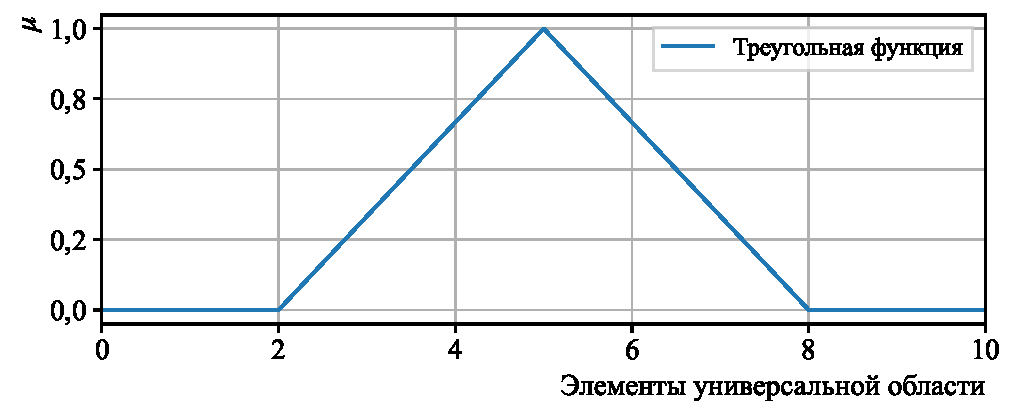
\includegraphics[]{part3/membership_function.pdf}
	\caption{Функция принадлежности нечеткого множества}
	\label{fig:membership_functions}
\end{figure}

Для формального описания процесса управления вводится понятие лингвистической переменной,
определяемой кортежем из пяти базовых элементов
\begin{equation}
	\langle \beta, T(\beta), X, G, M \rangle,
\end{equation}
где $\beta$ -- наименование лингвистической переменной;
$T(\beta)$ -- терм-множество значений, представляющее собой названия нечетких переменных;
$X$ -- универсальное множество, определяющее область значений рассматриваемой переменной;
$G$ -- синтаксические правила, порождающие названия значений лингвистической переменной;
$M$ -- семантические правила, задающие функции принадлежности нечетких термов.
\nomenclature{$\beta$}{Лингвистическая переменная\nomrefeqpage}
\nomenclature{$T(\beta)$}{Терм-множество значений\nomrefeqpage}
\nomenclature{$X$}{Универсальное множество\nomrefeqpage}
\nomenclature{$G$}{Синтаксические правила\nomrefeqpage}
\nomenclature{$M$}{Семантические правила\nomrefeqpage}


Для описания динамического состояния электропневматического привода
используются две основные лингвистические переменные:
\begin{equation}
	\beta = \left\{\beta_1, \beta_2\right\} = \left\{e, v\right\},
\end{equation}
где $e$ -- ошибка позиционирования;
$v$ -- скорость РО.

Дополнительно система может быть расширена путем включения информации о
давлениях в полостях пневмоцилиндра $p_1$ и $p_2$, что позволяет повысить
качество управления за счет учета термодинамических процессов.

Для ошибки позиционирования определяется следующая структура:
\begin{equation}
	\beta_1 = \text{<<ошибка позиционирования>>}.
\end{equation}

\begin{equation}
	T(\beta_1) =\begin{cases}
		\text{Отрицательная большая}; \\
		\ldots                        \\
		\text{Нулевая}     ;          \\
		\ldots                        \\
		\text{Положительная большая},
	\end{cases}
\end{equation}
при

\begin{equation}
	X_1 = [-x_{\text{max}}, x_{\text{max}}],
\end{equation}
где $x_{\text{max}}$ -- максимально возможное отклонение от заданного положения.

Синтаксические правила $G$ в данном случае определяют способы формирования составных термов:
\begin{equation}
	\text{G}: \text{знак} + \text{размер},
\end{equation}
где <<знак>> $\in$ {Отрицательная, Положительная}; <<размер>> $\in$ {Малая, Средняя, Большая}

Семантические правила $M$ устанавливают соответствие между термами и их функциями принадлежности:
\begin{equation}
	M: T(\beta_1) \rightarrow {\mu_i(x) | x \in X_1}.
\end{equation}

Аналогично для скорости изменения ошибки:
\begin{equation}
	\beta_2 = \text{<<скорость>>}.
\end{equation}

\begin{equation}
	T(\beta_2) =\begin{cases}
		\text{Отрицательная большая}; \\
		\ldots                        \\
		\text{Нулевая} ;              \\
		\ldots                        \\
		\text{Положительная большая},
	\end{cases}
\end{equation}

\begin{equation}
	X_2 = [-v_{\text{max}}, v_{\text{max}}],
\end{equation}
где $v_{\text{max}}$ -- максимально допустимая скорость.

На рисунке \ref{fig:linguistic_variable_structure} представлена структура лингвистической переменной
<<ошибка позиционирования>> с
7 термами на универсальном множестве $X$ от $-0,2$ до $0,2$.

\begin{figure}[ht]
	\centering
	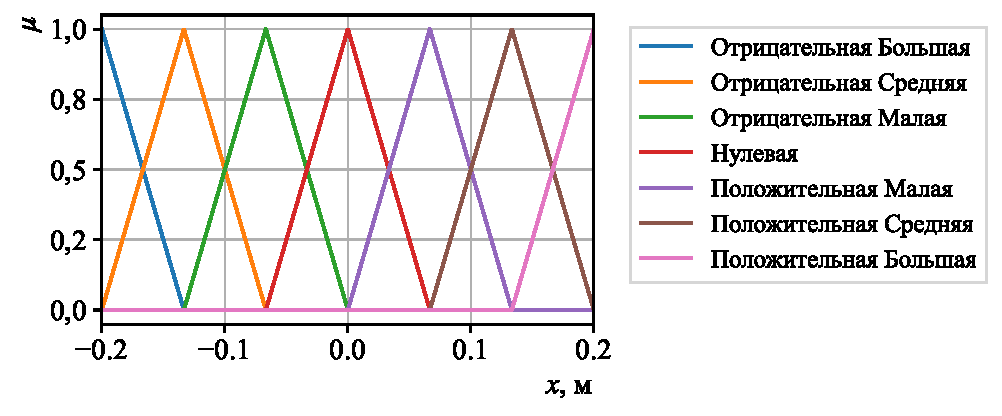
\includegraphics{part3/position_error_membership_functions.pdf}
	\caption{Структура лингвистической переменной}
	\label{fig:linguistic_variable_structure}
\end{figure}

Для каждого терма лингвистической переменной определяется функция принадлежности,
которая может быть представлена в различных формах,
как показано на рисунке \ref{fig:membership_functions_types}.
Наиболее распространенными являются:

Треугольная функция принадлежности:
\begin{equation}
	\mu_A(x; a, b, c) = \max\left(\min\left(\frac{x-a}{b-a}, \frac{c-x}{c-b}\right), 0\right).
\end{equation}

Гауссова функция принадлежности:
\begin{equation}\label{eq:gaussian_membership}
	\mu_A(x; c, \sigma) = \exp\left(-\frac{(x-c)^2}{2\sigma^2}\right).
\end{equation}

Z-образная функция принадлежности:
\begin{equation}\label{eq:z_membership}
	\mu_A(x; a, b) = \max\left(\min\left(\frac{x-a}{b-a}, 1\right), 0\right).
\end{equation}

Трапецеидальная функция принадлежности:
\begin{equation}
	\mu_A(x; a, b, c, d) = \max\left(\min\left(\frac{x-a}{b-a}, 1, \frac{d-x}{d-c}\right), 0\right).
\end{equation}

\begin{figure}[ht]
	\centering
	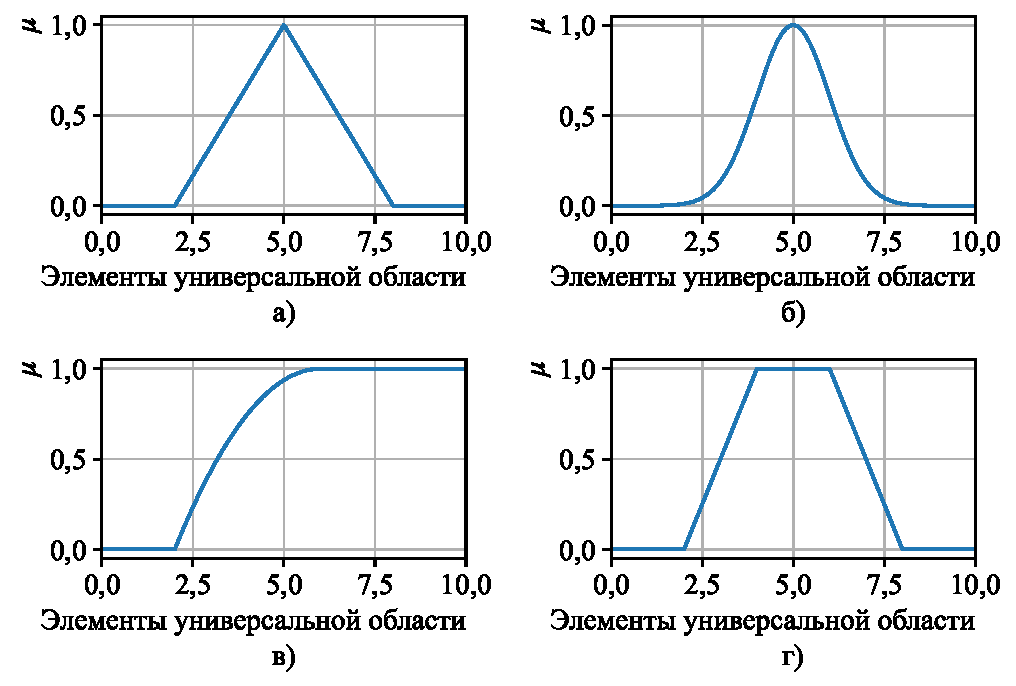
\includegraphics{part3/membership_functions.pdf}
	\caption{Типы функций принадлежности:\\
		а) треугольная; б) гауссова; в) z-образная; г) трапецеидальная}
	\label{fig:membership_functions_types}
\end{figure}

Важным аспектом определения лингвистической переменной является выбор
количества термов и их расположения
на универсальном множестве. При этом должны выполняться условия полноты:

\begin{equation}
	\forall x \in X: \sum_{i=1}^n \mu_i(x) > 0,
\end{equation}
и непротиворечивости:

\begin{equation}
	\forall x \in X: \sum_{i=1}^n \mu_i(x) \leq n,
\end{equation}
где $n$ -- количество термов.

База правил нечеткого вывода формируется на основе экспертных знаний
и представляется в виде продукционных правил согласно выражению \ref{eq:fuzzy_rule}. Такие правила как правило,
можно представить в табличном виде согласно рисунку \ref{fig:fuzzy_rules}:

\begin{equation}\label{eq:fuzzy_rule}
	R_i: \text{ЕСЛИ } e \text{ есть } A_i \text{ И } \dot{e} \text{ есть } B_i \text{ ТО } u \text{ есть } C_i.
\end{equation}

\begin{figure}[ht]
	\centering
	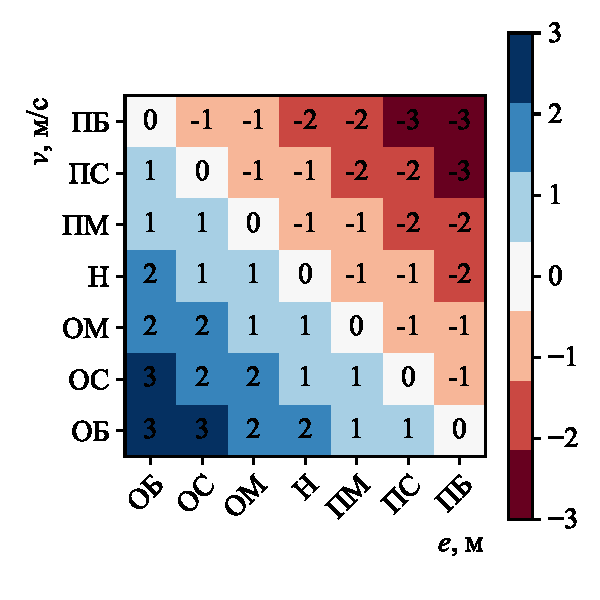
\includegraphics[]{part3/rule_base.pdf}
	\caption{Пример матрицы правил нечеткого вывода для электропневматического привода}
	\label{fig:fuzzy_rules}
\end{figure}

Процесс нечеткого логического вывода в разработанной системе управления реализуется в
соответствии с алгоритмом Мамдани, который включает последовательность
взаимосвязанных этапов преобразования информации, представленных на рисунке \ref{fig:fuzzy_inference}. Данный алгоритм
обеспечивает преобразование входных четких значений в выходные управляющие воздействия посредством
следующей математической процедуры.

На начальном этапе осуществляется фаззификация входных переменных, при которой определяется
степень принадлежности входных значений к различным нечетким множествам:
\begin{equation}
	\alpha_{ij} = \mu_{A_i}(e_j),
\end{equation}
где $\alpha_{ij}$ -- степень принадлежности входного значения $e_j$ к нечеткому множеству $A_i$;
$\mu_{A_i}(\cdot)$ - функция принадлежности соответствующего нечеткого множества.
\nomenclature{$\alpha_{ij}$}{Степень принадлежности входного значения $e_j$ к нечеткому множеству $A_i$\nomrefeqpage}
\nomenclature{$\mu_{A_i}(\cdot)$}{Функция принадлежности соответствующего нечеткого множества \nomrefeqpage}

Далее производится агрегирование подусловий в правилах нечеткого вывода путем
определения минимального значения степеней принадлежности:
\begin{equation}
	\alpha_i = \min(\alpha_{i1}, \alpha_{i2}),
\end{equation}
где $\alpha_i$ -- степень выполнения i-го правила нечеткой базы знаний.

На этапе активизации подзаключений формируются усеченные
функции принадлежности выходных лингвистических переменных:
\begin{equation}
	\mu'i(y) = \min(\alpha_i, \mu{C_i}(y)),
\end{equation}
где $\mu_{C_i}(y)$ -- функция принадлежности заключения i-го правила.

Аккумуляция заключений производится посредством объединения всех
усеченных функций принадлежности с использованием операции максимума:
\begin{equation}
	\mu_\Sigma(y) = \max_{i=1,m}\mu'_i(y).
\end{equation}

Заключительным этапом является дефаззификация результирующего
нечеткого множества, осуществляемая методом центра тяжести:
\begin{equation}
	y^* = \frac{\displaystyle\int\limits_{-\infty}^{+\infty} y\mu_\Sigma(y)dy}{\displaystyle\int\limits_{-\infty}^{+\infty} \mu_\Sigma(y)dy},
\end{equation}
где $y^*$ -- четкое значение выходной переменной, определяемое как центр тяжести площади под кривой
результирующей функции принадлежности $\mu_\Sigma(y)$.
\nomenclature{$y^*$}{Четкое значение выходной переменной, определяемое как центр тяжести площади под кривой результирующей функции принадлежности $\mu_\Sigma(y)$\nomrefeqpage}
В практической реализации пределы интегрирования ограничиваются областью определения
выходной переменной $[y_{min}, y_{max}]$, что обусловлено конечностью носителя нечеткого множества.

\begin{figure}[ht]
	\centering
	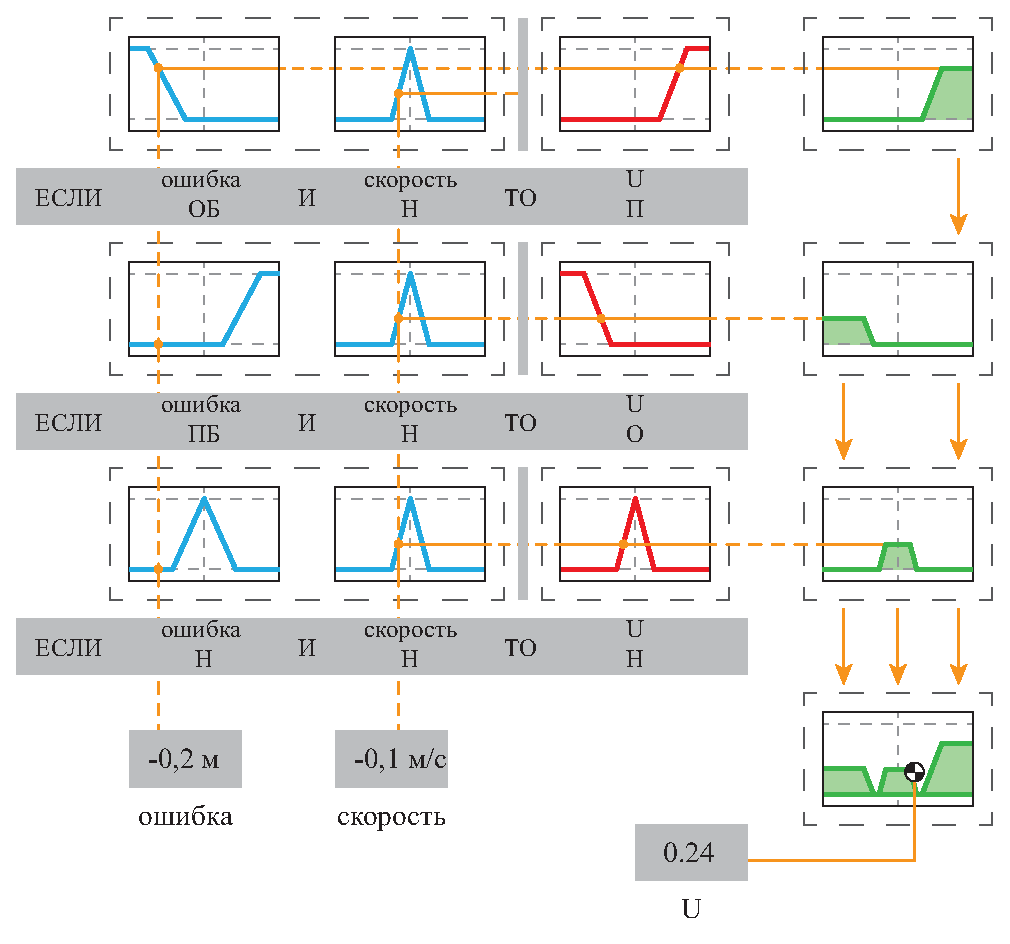
\includegraphics{part3/Мамдани.eps}
	\caption{Алгоритм Мамдани}
	\label{fig:fuzzy_inference}
\end{figure}

После выполнения дефаззификации осуществляется преобразование четкого значения управляющего воздействия
$y^*$ в дискретные режимы работы электропневматического привода посредством пороговой функции:
\begin{equation}
	\mathbf{u}(y^*) = \begin{cases}
		[1,0,0,1], & y^ \geq \varepsilon_2;                   \\
		[1,0,0,0], & \varepsilon_1 < y^* \leq \varepsilon_2;  \\
		[0,0,0,0], & |y^| \leq \varepsilon_1;                 \\
		[0,0,1,0], & -\varepsilon_2 < y^ \leq -\varepsilon_1; \\
		[0,1,1,0], & y^* \leq -\varepsilon_2,
	\end{cases}
\end{equation}
где $\varepsilon_1$, $\varepsilon_2$ ($\varepsilon_1 < \varepsilon_2$) -- пороговые значения, определяющие
границы переключения между режимами работы привода.
Данное преобразование обеспечивает формирование дискретных
управляющих воздействий на электромагнитные распределители в зависимости от
величины выходного сигнала нечеткого регулятора. При этом выбор
режима работы осуществляется таким образом, чтобы обеспечить плавное
изменение управляющего воздействия при переходе между различными состояниями системы.


\subsection*{Синтез нечеткого регулятора для пневмопривода с дискретными распределителями}\label{subsec:ch3/sec4/sub2}

Разработка матрицы правил нечеткой логики основывается на системном
анализе динамики пневмопривода. Процесс формирования базы правил можешь быть представлен
следующей последовательностью действий.
Первоначально определяются входные лингвистические переменные, как было показано в ранее, в данном случае это ошибка позиционирования $e$ и скорость $v$.

Далее происходит фаззификация входных переменных с использованием следующих термов:
\begin{enumerate}
	\item для ошибки: {ОБ (отрицательная большая),
	      ОМ (отрицательная малая),
	      Н (нулевая),
	      ПМ (положительная малая),
	      ПБ (положительная большая)};

	\item для скорости: {ОБ (отрицательная большая),
	      ОМ (отрицательная малая),
	      Н (нулевая),
	      ПМ (положительная малая),
	      ПБ (положительная большая)}.
\end{enumerate}

А так же определение функций принадлежности для каждого терма, согласно таблице
\ref{tab:operation_modes}. В качестве функции принадлежности для крайних термов используется Z-образная функция (\ref{eq:z_membership}),
а для промежуточных термов применяется функция Гаусса (\ref{eq:gaussian_membership}).

На рисунке \ref{fig:membership_functions_concrete} представлены функции принадлежности
для ошибки позиционирования и скорости соответственно.

\begin{figure}[ht]
	\centering
	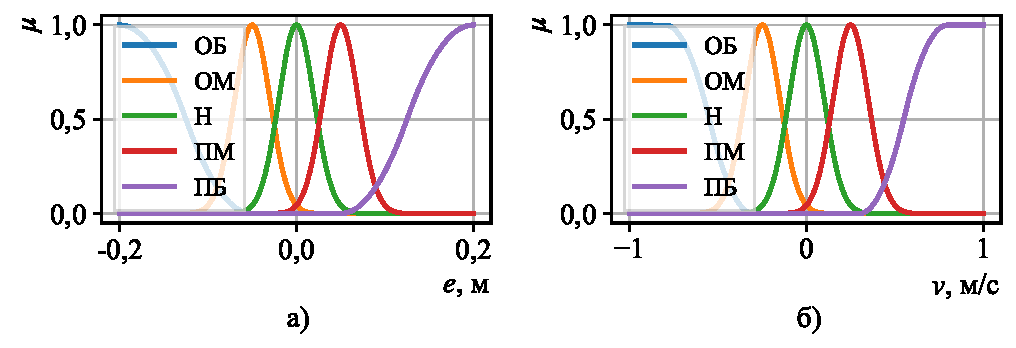
\includegraphics{part3/membership_functions_concrete.pdf}
	\caption{Функции принадлежности для ошибки позиционирования и скорости}
	\label{fig:membership_functions_concrete}
\end{figure}

Последним этапом происходит формирование базы правил нечеткого вывода, которая представляется
в виде матрицы, как показано на рисунке \ref{fig:fuzzy_rules}.

При разработке базы правил для нечеткого управления пневмоприводом
необходимо учитывать физические процессы, происходящие в системе.
Рассмотрим принцип формирования правил, основываясь на анализе
динамики пневмопривода.

При большой отрицательной ошибке, когда требуется движение влево,
учитываются различные физические состояния системы. В случае,
когда система уже движется влево с высокой скоростью, сохраняется
интенсивное управляющее воздействие, поскольку направление движения
соответствует требуемому. При замедлении движения влево применяется
умеренное воздействие для поддержания контролируемого движения.
Если система находится в состоянии покоя, осуществляется плавный
запуск движения для предотвращения резких динамических нагрузок.
В ситуации движения в неверном направлении (вправо) формируется
максимальное тормозящее усилие для изменения направления движения.

При малой отрицательной ошибке особое внимание уделяется
плавности движения. В случае быстрого движения влево начинается
постепенное торможение для предотвращения перерегулирования.
При медленном движении система переводится в режим удержания
позиции. Если наблюдается движение в неверном направлении,
формируется умеренное корректирующее воздействие.

В области нулевой ошибки основной задачей становится стабилизация
положения. При наличии остаточной скорости формируется тормозящее
усилие, пропорциональное скорости движения. В состоянии покоя все
распределители закрываются для минимизации расхода воздуха и
предотвращения автоколебаний.

Для малой положительной ошибки принципы формирования правил
аналогичны случаю малой отрицательной ошибки, но с противоположным
направлением воздействий. При большой положительной ошибке
логика управления зеркально отражает случай большой отрицательной ошибки.

Особое внимание при формировании правил уделяется учету сжимаемости
воздуха и существенного запаздывания между моментом переключения
распределителей и изменением давления в полостях цилиндра. Это
реализуется путем введения упреждающего торможения при высоких
скоростях движения. Также учитывается нелинейный характер изменения
давления в полостях цилиндра и влияние сил трения.

Каждое правило в базе формируется исходя из необходимости
обеспечения плавного движения с минимальным количеством
переключений распределителей при сохранении требуемого
быстродействия системы. При этом интенсивность управляющих
воздействий градуируется таким образом, чтобы обеспечить
оптимальное соотношение между скоростью реакции системы и
точностью позиционирования.

В результате получается база правил, представленная на рисунке \ref{fig:concrette_fuzzy_rules}, а результаты моделирования на \ref{fig:fuzzy_transient}.

\begin{figure}[ht]
	\centering
	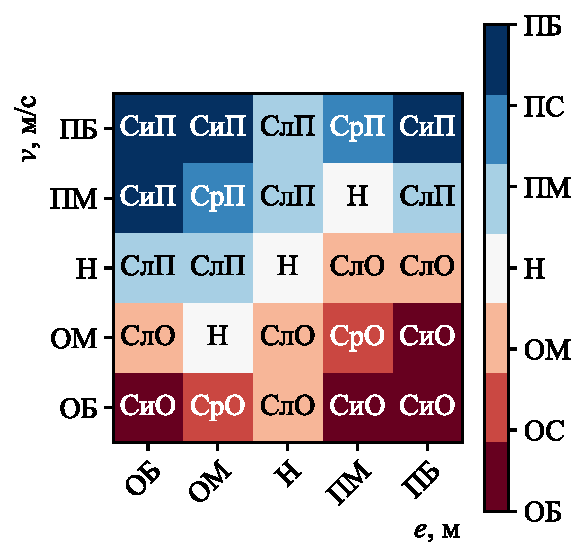
\includegraphics{part3/rule_base_concrete.pdf}
	\caption{База правил по конкретному описанию динамики пневмопривода}
	\label{fig:concrette_fuzzy_rules}
\end{figure}

\begin{figure}[ht]
	\centering
	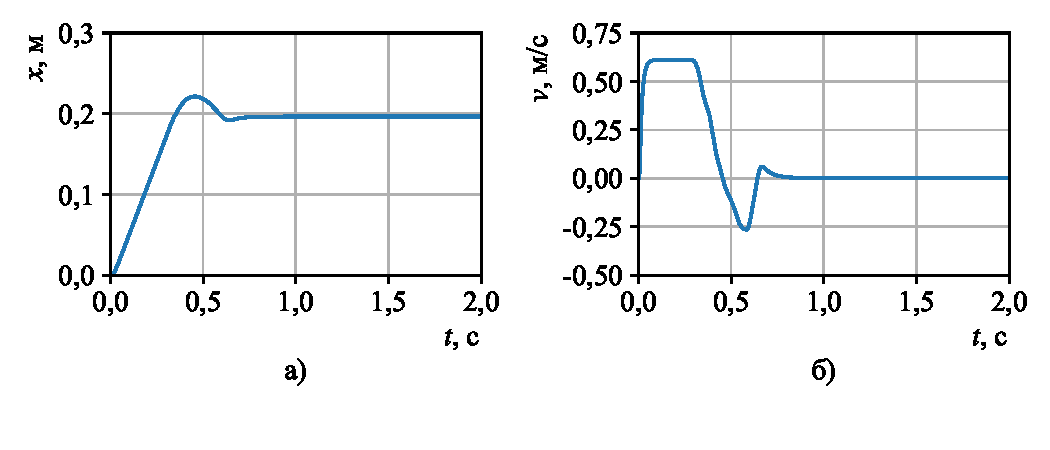
\includegraphics{part3/fuzzy_control.pdf}
	\caption{Переходной процесс для представленного нечетко-логического контроллера }
	\label{fig:fuzzy_transient}
\end{figure}

Важной особенностью разработанного нечеткого регулятора является адаптивное изменение интенсивности управляющего
воздействия в зависимости от текущего состояния системы, что позволяет минимизировать количество переключений распределителей при
сохранении удовлетворительного качества переходного процесса.
